% Quick start guide
\documentclass[aspectratio=169]{beamer}

\usepackage{minted}
\usepackage{xcolor}
\definecolor{LightGray}{gray}{0.9}

\usetheme {default}

\graphicspath{{images/}{\main/images/}}

% Title page details
\title {git training}
\subtitle{git, workflows, github}
%\author{latex-beamer.com}
%\institute{KUNBUS GmbH}
%\date{\today}

\renewcommand{\footnotesize}{\tiny}

% Image Logo
\logo{
\includegraphics[width=2.5cm]{kunbus-logo.png}} 

\begin{document}

\begin{frame}
% Print the title page as the first slide
\titlepage
\end{frame}

% Presentation outline
\begin{frame}{Outline}
    \tableofcontents
\end{frame}

\section{What is a VCS?}
\begin{frame}{What is a VCS?}
\begin{itemize}
    \item Tracks changes
    \item Creates a history over the changes
    \item Provides traceability
    \item Provides attribution
\end{itemize}
\end{frame}

\begin{frame}{Centralized VCS}{Centralized vs. Distributed VCS}
\begin{figure}
    \centering
    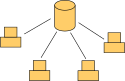
\includegraphics[width=\textwidth,height=0.6\textheight,keepaspectratio]{01_centralized_vcs}
\end{figure}
\end{frame}

\begin{frame}{Distributed VCS}{Centralized vs. Distributed VCS}
\begin{figure}
    \centering
    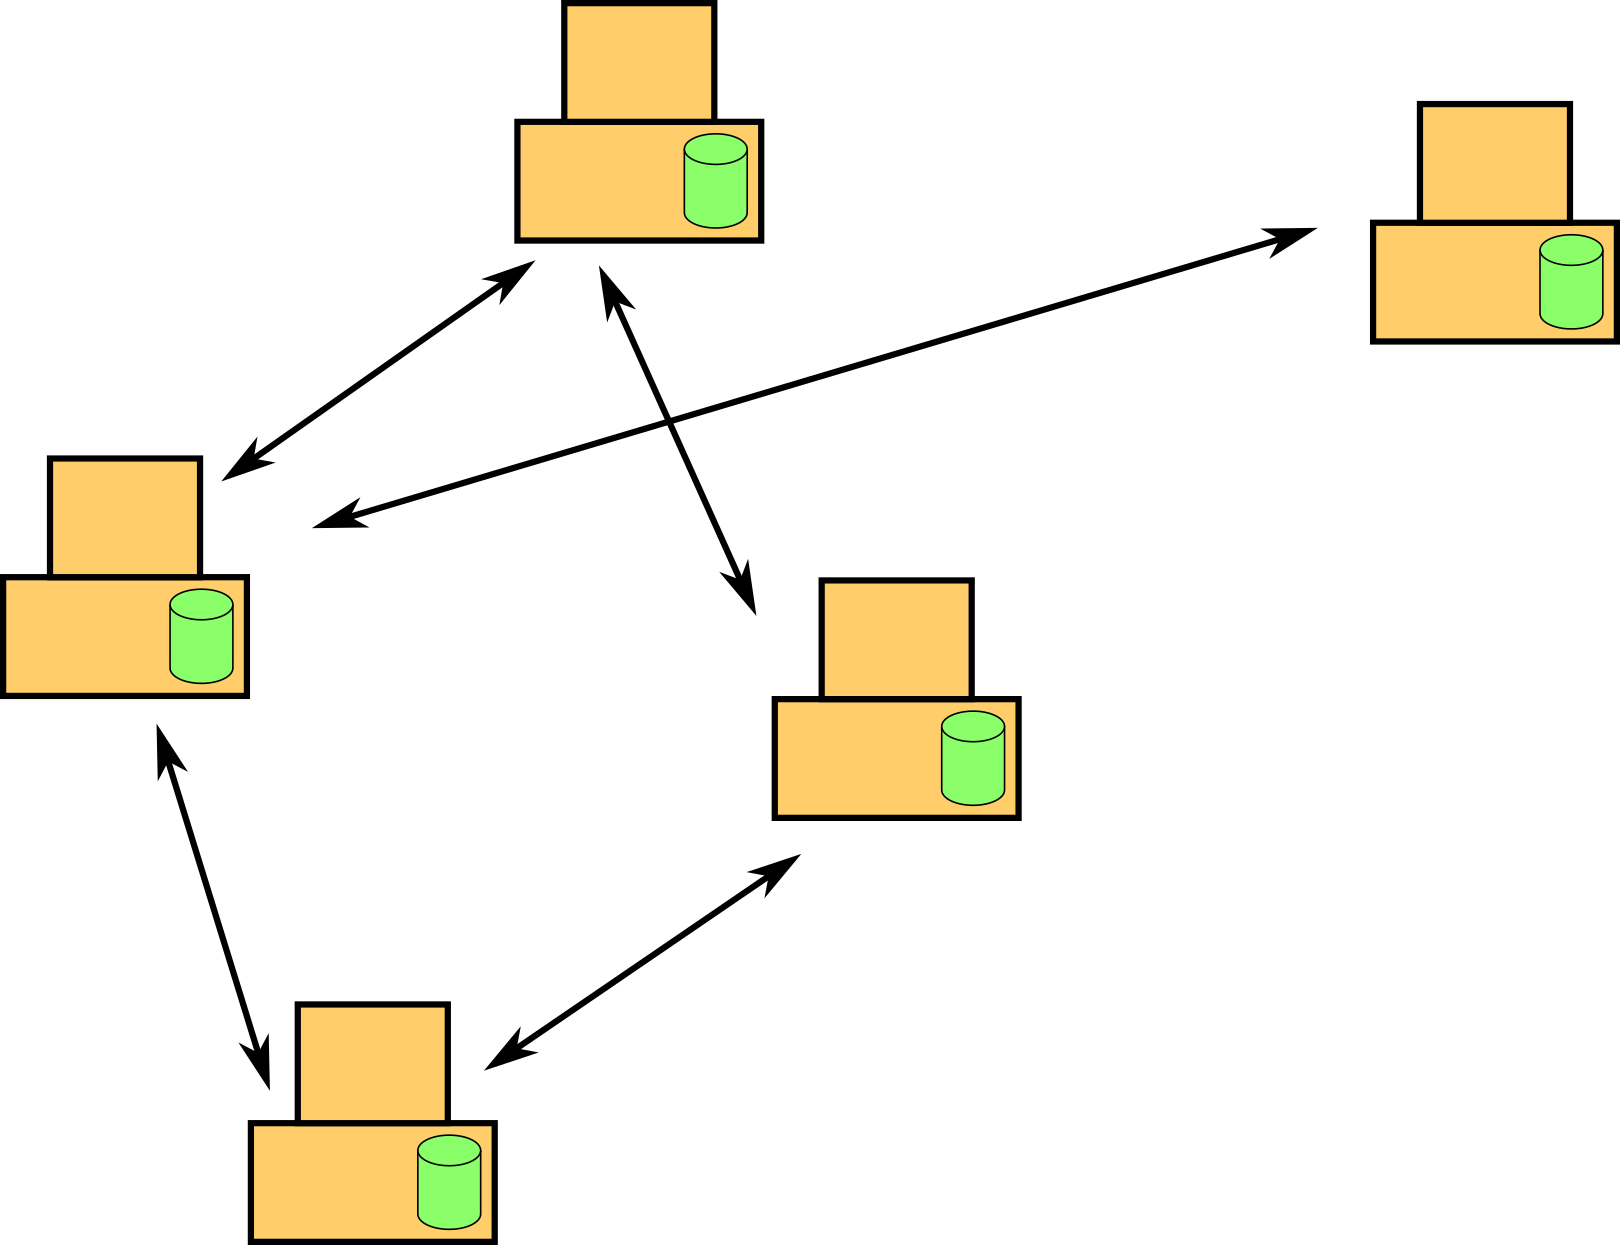
\includegraphics[width=\textwidth,height=0.6\textheight,keepaspectratio]{02_distributed_vcs}
\end{figure}
\end{frame}

\begin{frame}{Deltas}{Deltas vs. Snapshots}
\begin{figure}
    \centering
    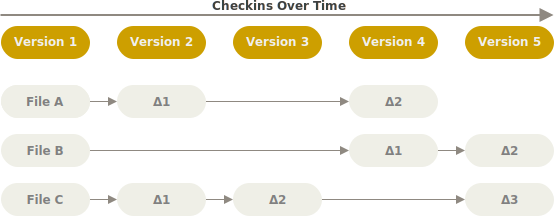
\includegraphics[width=\textwidth,height=0.6\textheight,keepaspectratio]{deltas}
    \caption{
        Pro Git: 1.3 Getting Started - What is Git?\footnote{\url{https://git-scm.com/book/en/v2/Getting-Started-What-is-Git\%3F}}
    }
\end{figure}
\end{frame}

\begin{frame}{Snapshots}{Deltas vs. Snapshots}
\begin{figure}
    \centering
    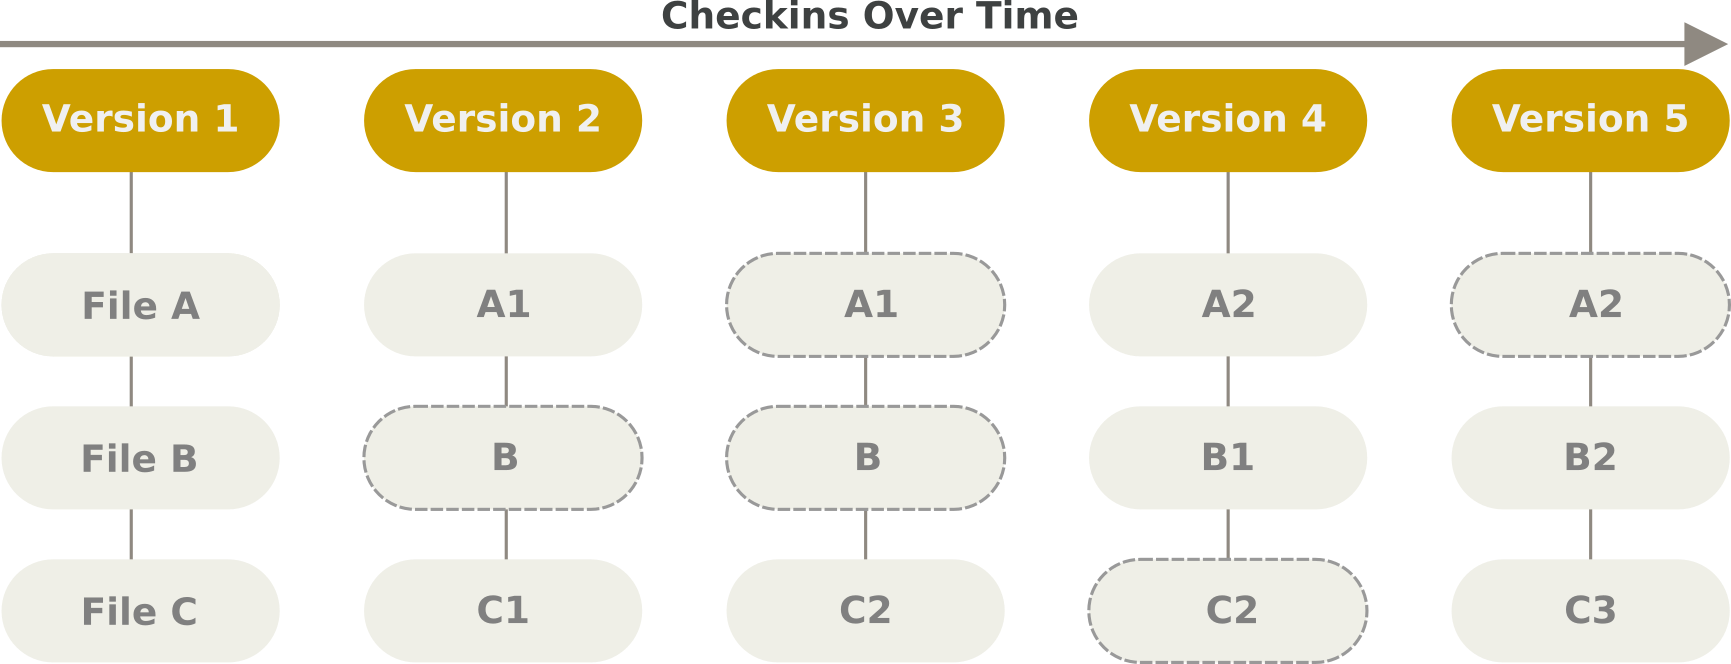
\includegraphics[width=\textwidth,height=0.6\textheight,keepaspectratio]{snapshots}
    \caption{
        Pro Git: 1.3 Getting Started - What is Git?\footnote{\url{https://git-scm.com/book/en/v2/Getting-Started-What-is-Git\%3F}}
    }
\end{figure}
\end{frame}

\section{How does Git work?}
\begin{frame}[fragile]{Every thing is a Hash}{How does Git Work?}
\begin{minted}[bgcolor=LightGray,fontsize=\small]{text}
$ sha1sum kunbus-logo.png 
c263869cf482a5d5d4262170ec242f8f13fc3def  kunbus-logo.png
$ ls -sh kunbus-logo.png 
352K kunbus-logo.png
\end{minted}
\begin{itemize}
    \item A file is an \emph{object} with a \emph{hash} and a \emph{size}
    \item Everything is identified by its hash, not only file objects
\end{itemize}
\end{frame}

\begin{frame}{Git is a Tree of Hashes}{How does Git Work?}
\begin{figure}
    \centering
    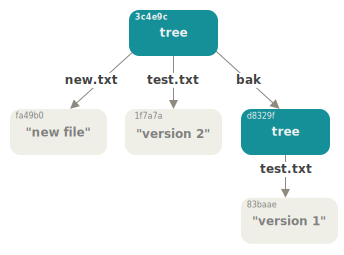
\includegraphics[width=\textwidth,height=0.6\textheight,keepaspectratio]{data-model-2}
    \caption{
        Pro Git: 10.2 Git Internals - Git Objects\footnote{\url{https://git-scm.com/book/en/v2/Git-Internals-Git-Objects}}
    }
\end{figure}
\end{frame}

\begin{frame}{Git is a Tree of Trees of Hashes}{How does Git Work?}
\begin{figure}
    \centering
    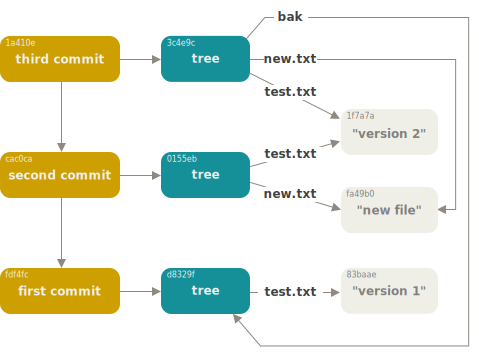
\includegraphics[width=\textwidth,height=0.6\textheight,keepaspectratio]{data-model-3}
    \caption{
        Pro Git: 10.2 Git Internals - Git Objects\footnote{\url{https://git-scm.com/book/en/v2/Git-Internals-Git-Objects}}
    }
\end{figure}
\end{frame}

\section{The Basics}
\begin{frame}[fragile]{Getting a Git Repository}{Git Basics}
\begin{itemize}
    \item Create an directory
    \item Call \verb|git init| inside the directory
\end{itemize}
\begin{minted}[bgcolor=LightGray,fontsize=\small]{text}
$ mkdir my_project
$ cd my_project
$ git init
Initialized empty Git repository in /home/user/my_project/.git/
\end{minted}
\begin{itemize}
    \item This creates a local repository
    \item It is contained in the \verb|.git| directory under the \verb|my_project| directory
\end{itemize}
\end{frame}

\begin{frame}[fragile]{Getting a Git Repository}{Git Basics}
\begin{itemize}
    \item With \verb|git clone| we can get a remote repository
\end{itemize}
\begin{minted}[bgcolor=LightGray,fontsize=\small]{text}
$ git clone https://github.com/libgit2/libgit2
Cloning into 'libgit2'...
remote: Enumerating objects: 119184, done.
remote: Counting objects: 100% (119184/119184), done.
remote: Compressing objects: 100% (32744/32744), done.
remote: Total 119184 (delta 84532), reused 119074 (delta 84433), pack-r...
Receiving objects: 100% (119184/119184), 61.22 MiB | 7.21 MiB/s, done.
Resolving deltas: 100% (84532/84532), done.
\end{minted}
\begin{itemize}
    \item This creates the directory \verb|libgit2|
    \item A git repository (\verb|.git|) is create inside the directory
    \item The git repository contains a \emph{complete} copy of the remote repository
\end{itemize}
\end{frame}

\begin{frame}[fragile]{Recording Changes to the Repository}{Git Basics}
\begin{itemize}
    \item Files in the working tree can be in four states:
    \begin{itemize}
        \item unmodified
        \item modified
        \item untracked
        \item staged
    \end{itemize}
\end{itemize}
\end{frame}

\begin{frame}{Recording Changes to the Repository}{Git Basics}
\begin{block}{unmodified}
    Files which are under control of git. All changes have been recorded to the
    history. No additional changes have been made to the files.
\end{block}
\begin{block}{modified}
    Files which are under control of git. Files that have been changed since
    the last time the changes to the file have been recorded to the history.
\end{block}
\end{frame}


\begin{frame}{Recording Changes to the Repository}{Git Basics}
\begin{block}{untracked}
	Files which are in the working tree but are not under the control of git.
	They don't exist in the history. This can be new files or build artifacts
	which should not be included in the git repository.
\end{block}
\begin{block}{staged}
	Files which are marked to be recorded to the history. Changes to files files
	in modified stage need to be staged before they can be recorded to the
	history. Also untracked files need to be staged before the can be recorded to
	the history.
\end{block}
\end{frame}

\begin{frame}{Recording Changes to the Repository}{Git Basics}
\begin{figure}
    \centering
    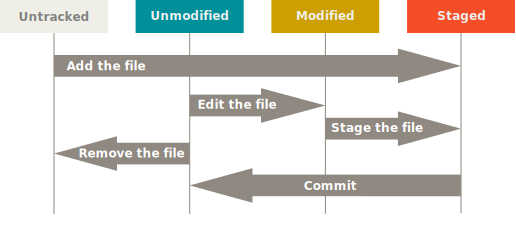
\includegraphics[width=\textwidth,height=0.6\textheight,keepaspectratio]{lifecycle}
    \caption{
        Pro Git: 12.2 Git Basics - Recording Changes to the Repository\footnote{\url{https://git-scm.com/book/en/v2/Git-Basics-Recording-Changes-to-the-Repository}}
    }
\end{figure}
\end{frame}

\section{Not so Basic}
\section{Workflows}
\section{Github}

\end{document}
